\documentclass{beamer}

\usepackage{subfig}
\usepackage{hyperref}
\usepackage{csquotes}
\usepackage[Q=yes]{examplep}
\usepackage[dvipsnames]{xcolor}

\hypersetup{
    colorlinks=true,
    linkcolor=blue,
    filecolor=magenta,      
    urlcolor=cyan,
}

\mode<presentation> {
    \usetheme{Madrid}
}

\title[\textcolor{white}{Vim - Fun and Efficient}]{\huge Vim \\
    \large Making text editing fun and efficient
}

\author{Alec Gibson}
\institute[BlueCat]
{
    BlueCat Networks \\
    \medskip
    \textit{agibson@bluecatnetworks.com}
}
\date{November 24, 2020}

\begin{document}

\begin{frame}
    \titlepage % Print the title page as the first slide
\end{frame}

\begin{frame}
    \frametitle{Disclaimer}
    \small The target audience of this talk is not seasoned users of Vi-family editors (though you are more than welcome to stay if this describes you). Many of the features I will refer to as Vim features were Vi features first. I never used Vi, and clarifying when features were introduced in Vim's lineage is outside the scope of this talk. So for the purpose of this talk they are Vim features.\\
    \vspace{0.5cm}
    Furthermore, almost everything I say in this talk applies equally to Neovim as it does to Vim. Neovim is a fork of Vim with slightly tweaked default options, no Benevolent Dictator For Life, and which tends to implement new features more quickly. I personally use Neovim instead of Vim, but both operate extremely similarly.
\end{frame}

\begin{frame}
    \frametitle{About This Presentation}
    \begin{itemize}
	\item This presentation was created in Neovim 0.5.0 using the Beamer Latex package
	\item The source code is available at \url{https://github.com/alec-gibson/vim-fun-and-efficient}
	\item For discussions about Vim, please post in the company \#vim-geeks slack channel!
    \end{itemize}
\end{frame}

\begin{frame}
    \frametitle{Overview}
    \tableofcontents
\end{frame}

\section{About Vim}

\begin{frame}
    \frametitle{About Vim}
    \tableofcontents[currentsection]
\end{frame}

\begin{frame}
    \frametitle{What is Vim}
    \centerline{\large According to vim.org}
    \vspace{0.5cm}
    \small Vim is a highly configurable text editor built to make creating and changing any kind of text very efficient. It is included as \enquote{vi} with most UNIX systems and with Apple OS X.\\
    \vspace{0.5cm}
    Vim is rock stable and is continuously being developed to become even better. Among its features are:\\
    \begin{itemize}
	\item persistent, multi-level undo tree
	\item extensive plugin system
	\item support for hundreds of programming languages and file formats
	\item powerful search and replace
	\item integrates with many tools
    \end{itemize}
\end{frame}

\begin{frame}
    \centerline{\large Here are some important features I think were missed:}
    \vspace{0.5cm}
    \small
    \begin{itemize}
	\item Vim is very lightweight, meaning it runs smoothly on any modern computer and performs well over SSH.
	\item Vim's startup time is nearly instantaneous.
	\item Because Vim runs in a terminal it works nicely with other terminal utilities (like tmux), and you can pipe the output of scripts directly into Vim.
	\item Vim's configuration is scriptable, so you can define custom functions then use them in commands and keybindings.
	\item Once you learn Vim you can use it everywhere - its keybindings are supported in most other editors either natively or through plugins (including VSCode, Emacs, and IntelliJ to name a few)
    \end{itemize}
\end{frame}

\begin{frame}
    \centerline{\large And most importantly....}
    \vspace{0.5cm}
    \small \textbf{If you are not already using them, Vim's keybindings can teach you a new, more efficient way to edit text.}\\
\end{frame}

\begin{frame}
    \frametitle{Who Should Try Vim?}
    \centerline{\large You may appreciate Vim if you:}
    \vspace{0.5cm}
    \begin{itemize}
	\item Spend a large amount of your day editing plain text files (common in software development and IT)
	\item Make frequent use of your terminal emulator
	\item Appreciate the value of keyboard shortcuts for everything
	\item Like to customize your tools to suit your workflow
	\item \textbf{And especially} if you spend too much time making boring, repetitive edits
    \end{itemize}
\end{frame}

\section{A Minimal Vim Workflow}

\begin{frame}
    \frametitle{A Minimal Vim Workflow}
    \tableofcontents[currentsection]
\end{frame}

\begin{frame}[fragile]
    \frametitle{Modal Editing}
    \small
    \begin{block}{Modal Editing}
	Vim is a modal text editor, meaning keypresses in Vim perform different actions depending upon the editor's current \enquote{mode}.\\
    \end{block}
    When you edit a file in Vim, the editor starts in \enquote{normal} mode. This can confuse new users, because Vim's normal mode treats every key on the keyboard as a binding for a shortcut. To start off learning Vim, let's look at the smallest possible set of features you need to edit files.
\end{frame}

\begin{frame}[fragile]
    \frametitle{Basic Vim File Operations}
    \small
    \begin{itemize}
	\item To open a file in Vim, type \verb+vim {filename}+ in your terminal emulator.
	\item To change the current open file, type \verb+:e /path/to/file<CR>+.
	\item To save the current file, type \verb+:w<CR>+.
	\item Finally, to exit Vim type \verb+:q<CR>+.
    \end{itemize}
    \begin{block}{What's That CR Symbol?}
	\verb+<CR>+ is how you represent the Enter/Return key in Vim keybindings.
    \end{block}
    \begin{block}{Popular Variants}
	Popular variants of these commands include \verb+:wq<CR>+ to save and quit, and \verb+:wq!<CR>+ to force Vim to save and quit (ignoring any warnings while doing so).
    \end{block}
\end{frame}

\begin{frame}[fragile]
    \frametitle{Basic Vim Editing}
    \small
    The simplest (though probably the slowest) way to navigate a file in Vim is using the arrow keys. To make changes in the current file, press \verb+i+ to enter \enquote{insert} mode. In insert mode, keys behave the way they would in any other text editor - letter and number keys insert their corresponding characters, and \verb+<BS>+ (backspace) deletes the previous character. \\
    \vspace{0.5cm}
    If you want to run any of the file operations from the previous slide, just press \verb+<ESC>+ (escape) to return to normal mode first.
    \begin{block}{Using Your Mouse in Vim!?}
	It's true, Vim supports using your mouse. Just set the required option by typing \verb+:set mouse=a+ in normal mode.
    \end{block}
\end{frame}

\begin{frame}
    \small This is about as much of Vim as some people ever learn. It's enough to edit config files on servers over SSH (albeit slowly), or to use while setting up a minimal Linux installation on a PC. \\
    \vspace{0.5cm}
    However, if this was the most efficient way to edit files in Vim, \textbf{the editor would have died out long ago}.
\end{frame}

\section{Vim Can Do More}

\begin{frame}
    \frametitle{Vim Can Do More}
    \tableofcontents[currentsection]
\end{frame}

\begin{frame}[fragile]
    \frametitle{Why The Minimal Workflow Isn't Enough}
    \small
    The minimal Vim workflow I layed out is seriously inefficient. Here are a few of the more obvious reasons why:
    \begin{itemize}
	\item Using the mouse requires you to take your right hand off the keyboard
	\item Using the arrow keys requires you to take your right hand off the home row
	\item You can only move one character at a time using the arrow keys
	\item You can only delete one character at a time using \verb+<BS>+
	\item If your cursor is in the middle of some text, you have to move to the end before deleting it
	\item This workflow doesn't include any way to search the current file
	\item Repeated edits need to be executed manually each time
    \end{itemize}
    Vim's normal mode has features which solve all these issues.
\end{frame}

\begin{frame}[fragile]
    \frametitle{Movement Keybindings}
    \small
    \begin{block}{Problems}
	\begin{itemize}
	    \item Using the mouse requires you to take your right hand off the keyboard
	    \item Using the arrow keys requires you to take your right hand off the home row
	\end{itemize}
    \end{block}
    Vim solves these issues by using the keys \verb+h, j, k, and l+ as alternatives to the arrow keys while in normal mode. These behave in the following manner:
    \begin{description}
	\item[h] Move left one character
	\item[j] Move down one character
	\item[k] Move up one character
	\item[l] Move right one character
    \end{description}
    These are some of Vim's most well-known normal mode keybindings, and other programs which also support these keybindings often refer to them as \enquote{Vim keys}.
\end{frame}

\begin{frame}[fragile]
    \frametitle{Moving Longer Distances}
    \small
    \begin{block}{Problems}
	\begin{itemize}
	    \item You can only move one character at a time using the arrow keys
	\end{itemize}
    \end{block}
    Vim's normal mode contains many keybindings for moving more than one character at a time. Here are some I use frequently:
    \begin{itemize}
	\item w/b --- Move forward/back by one word at a time
	\item 0/\$ --- Move to the start/end of the current line
	\item \verb+<C-d>+/\verb+<C-u>+ --- Move down/up by half a screen at a time
    \end{itemize}
    \begin{block}{Useful Keybindings: f and F}
	Typing f\{character\} makes Vim search forward along the current line for your chosen character, and using F instead searches backwards. Pressing \enquote{;} makes Vim keep searching for the next occurrence, and pressing \enquote{,} makes Vim search in the opposite direction (very useful if you overshoot your target). This is often the fastest way to jump to a specific location in your current line.
    \end{block}
\end{frame}

\begin{frame}[fragile]
    \begin{block}{Repeating Movements Multiple Times}
	Most Vim commands allow you to prepend a number to multiply their effects. For example:
	\begin{itemize}
	    \item typing \verb+5j+ in normal mode moves your cursor down 5 lines.
	    \item typing \verb+3w+ moves your cursor forward 3 words
	    \item typing \verb+10fe+ moves your cursor to the tenth occurence of the character \enquote{e} following it on the current line
	\end{itemize}
    \end{block}
\end{frame}

\begin{frame}
    \frametitle{Keybindings for Editing}
\end{frame}

\begin{frame}[fragile]
    \frametitle{Deleting Chunks of Text}
    \begin{block}{Problems}
	\begin{itemize}
	    \item You can only delete one character at a time using \verb+<BS>+
	\end{itemize}
    \end{block}
\end{frame}

\begin{frame}
    \frametitle{Text Objects}
\end{frame}

\begin{frame}
    \frametitle{Searching}
\end{frame}

\begin{frame}
    \frametitle{Repeating Edits}
    Vim supports many ways to repeat edits. I'll discuss some of the other ones I use frequently in the \enquote{Power Tools} section of this talk.
\end{frame}

\begin{frame}
    \frametitle{Command-Line Mode}
\end{frame}

\begin{frame}
    \frametitle{Visual Mode}
\end{frame}

\begin{frame}
    \frametitle{How to Find Help}
\end{frame}

\section{Power Tools}

\begin{frame}
    \frametitle{Power Tools}
    \tableofcontents[currentsection]
\end{frame}

\begin{frame}
    \frametitle{The Jump List}
\end{frame}

\begin{frame}
    \frametitle{Registers and Macros}
\end{frame}

\begin{frame}
    \frametitle{Substitute and Global}
\end{frame}

\begin{frame}
    \frametitle{The Undo Tree}
\end{frame}

\begin{frame}
    \frametitle{Vimscript}
\end{frame}

\begin{frame}
    \frametitle{Execute and Normal}
\end{frame}

\section{File Navigation}

\begin{frame}
    \frametitle{File Navigation}
    \tableofcontents[currentsection]
\end{frame}

\begin{frame}
    \frametitle{Buffers, Windows and Tabs}
\end{frame}

\begin{frame}
    \frametitle{Argument, Location and Quickfix Lists}
\end{frame}

\begin{frame}
    \frametitle{Grep and Vimgrep}
\end{frame}

\begin{frame}
    \frametitle{Cdo, Ldo, Argdo}
\end{frame}

\begin{frame}
    \frametitle{Finding Files Quickly}
    NOTE: discuss fuzzy finder and file tree plugins here
\end{frame}

\section{Configuration}

\begin{frame}
    \frametitle{Configuration}
    \tableofcontents[currentsection]
\end{frame}

\begin{frame}
    \frametitle{Setting Options}
\end{frame}

\begin{frame}
    \frametitle{Keybindings and Abbreviations}
\end{frame}

\begin{frame}
    \frametitle{Functions and Custom Commands}
\end{frame}

\begin{frame}
    \frametitle{Automatic Commands}
\end{frame}

\begin{frame}
    \frametitle{Plugins}
\end{frame}

\section{Links for Further Learning}

\begin{frame}
    \frametitle{Links for Further Learning}
\end{frame}

\section{Goodbye}

\begin{frame}
    \centerline{\huge All Praise VI VI VI}
    \vspace{0.5cm}
    \centerline{\huge Editor of The Beast}
    \begin{figure}
	\centering
	\subfloat{{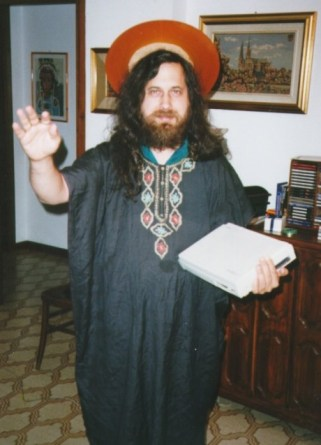
\includegraphics[width=0.3\linewidth]{saintignucius.jpg} }}% Created by Wouter van Oortmerssen
	\qquad
	\subfloat{{
\includegraphics[width=0.3\linewidth]{freebsd-daemon.png} }}% Created by Poul-Henning Kamp under the beer-ware license (https://svnweb.freebsd.org/base/head/share/examples/BSD_daemon/README?view=markup)
    \end{figure}
\end{frame}

\end{document} 
